% Companion Pandoc template: preserve the original CPB Beamer preamble and layout.
\documentclass[aspectratio=169,11pt,handout,xcolor=dvipsnames]{beamer}

\usepackage[utf8]{inputenc}
\usepackage[T1]{fontenc}
\graphicspath{{../}}
\makeatletter
\def\input@path{{../}}
\makeatother
\usepackage{cpb-beamer} % Reuse the original CPB style from the parent folder.
\usepackage[dutch,english]{babel}  % Gebruik [english, dutch]{babel} voor nederlandse datumnotatie
\usepackage{booktabs}
\usepackage{colortbl}
\usepackage{array}
\newcommand{\mypos}[2]{\tikz[remember picture]{\node[inner sep=0pt, anchor=base](#2){#1};}}
\newcommand{\myund}{}
\usepackage{pgfplots}
\pgfplotsset{compat=1.18}
\usepackage{adjustbox}  % voor clippen van achtergrondafbeelding
\usepackage{setspace}
\usepackage{soul}
\usepackage{natbib} % voor using bibliographystyle amcg
\usepackage{bm}
\usepackage{amsmath,amsfonts,eqnarray}
\usepackage{amssymb,dsfont,bbold}
\usepackage{changepage}
\usepackage{nicefrac}
\usepackage{multirow}
\usepackage{subcaption}


\title[Short title]{Layout presentations CPB}
\author{M. Kattenberg based on A. Schmidt CPB-style file following J.
Tijm's template}
\disclaimer{With a lot of help from Codex}
\date{\today}
\cpbfooter{J. Tijm, A. Schmidt}
\cpbtitelafbeelding{Images/cover_bg.png} % Titel figuur

\providecommand{\tightlist}{}
\begin{document}
\cpbtitelframe

\begin{frame}{}
\label{teaser}
\vspace{1cm}

\begin{block}{\centering Task}
\centering A block
\end{block}

\pause
\vspace{1cm}
\begin{itemize}
\tightlist
\item
  A list:
  \begin{itemize}
  \tightlist
  \item
    Bullet 1
  \item
    \pause Bullet 2
  \end{itemize}
\end{itemize}
\end{frame}

\cpbinhoudframe{\begin{itemize}
\tightlist
\item
  A list:
  \begin{itemize}
  \tightlist
  \item
    Bullet 1
  \item
    \pause Bullet 2
  \end{itemize}
\end{itemize}}

\cpbsectie{Section}{}

\begin{frame}{A title in the frame}
\label{a-title-in-the-frame}
\begin{itemize}
\tightlist
\item
  References can be used using the references.bib file.
  \begin{itemize}
  \tightlist
  \item
    You can cite \cite{lundberg2017} or \citep{lundberg2017}
  \end{itemize}
\item
  We recommend adding the Figures in the Figures folder (you can also add subfolders if needed).
  \begin{itemize}
  \tightlist
  \item
    Reference by using Figure \ref{fig:example_figure}
  \item
    If the figures and tables order change, the numbers are automatically updated.
  \end{itemize}
\end{itemize}

\begin{figure}[H]
\centering
\vspace{-0.5cm}
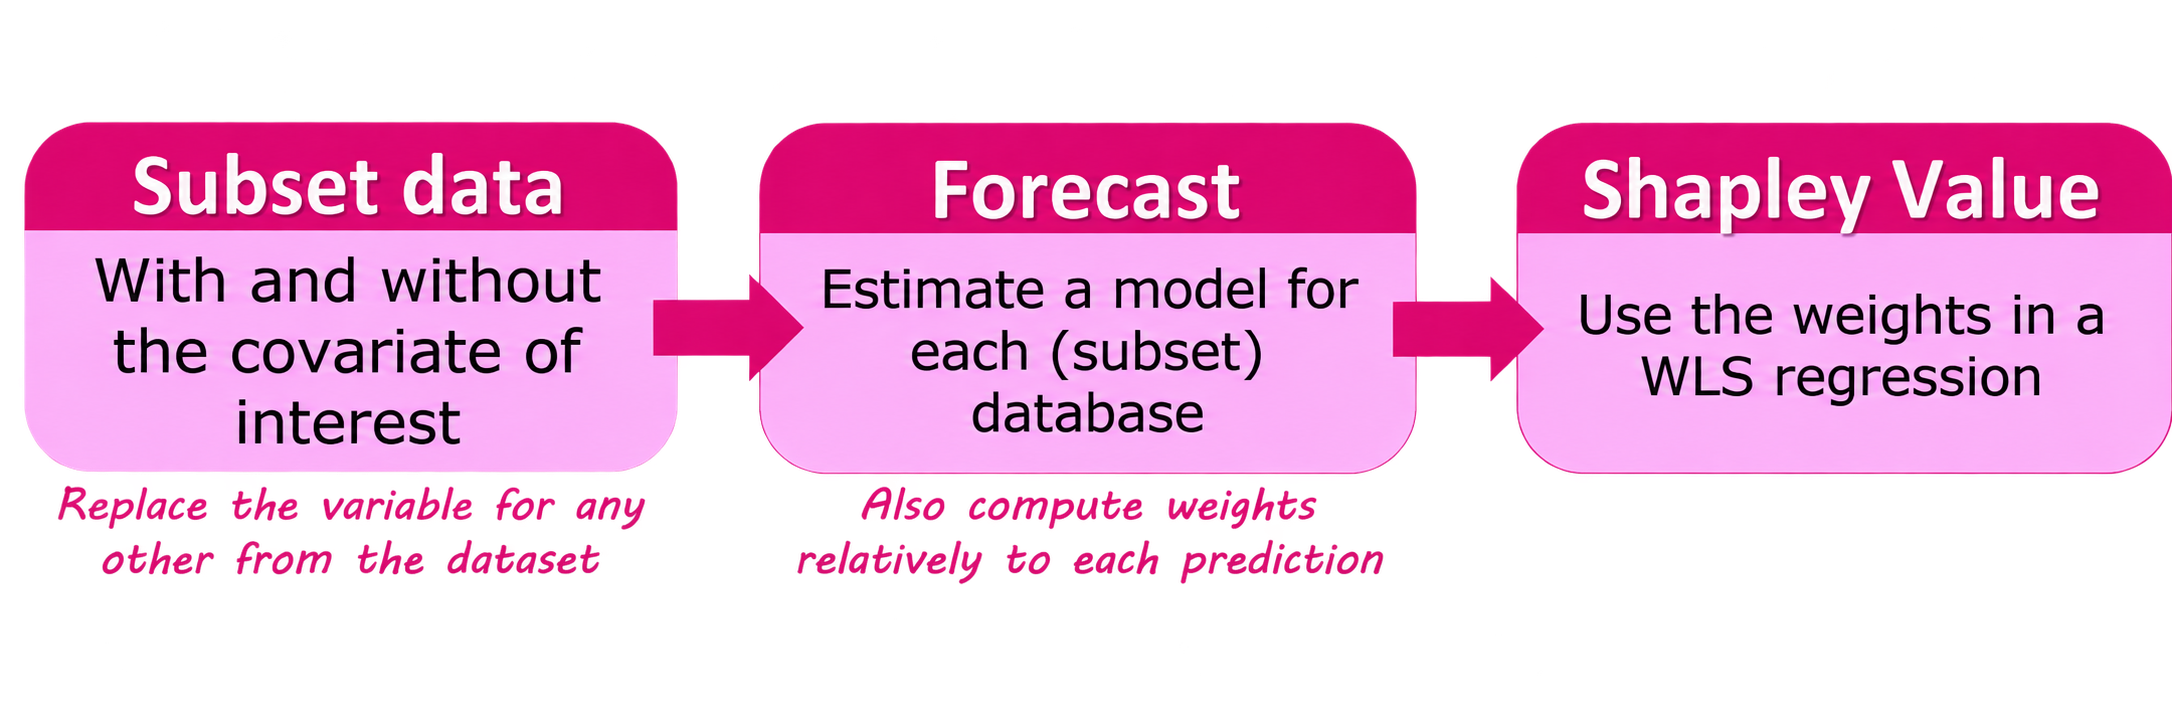
\includegraphics[scale=0.12]{../Figures/SHAP2.png}
\vspace{-0.5cm}
\caption{\scriptsize{Example of a Figure}}
\label{fig:example_figure}
\end{figure}
\end{frame}

\begin{frame}{Custom LaTeX diagrams}
\label{custom-latex-diagrams}
\vspace{1cm}

  % Maximum 4 boxes
  \begin{figure}
    \centering
    \resizebox{0.6\linewidth}{!}{%
    \cpbdiagram{magenta}{4}{%
      \cpbdiagramitem
        {Box 1}
        {Text 1}
        {Caption 1}
      \cpbdiagramitem
        {Box 2}
        {Text 2}
        {Caption 2}
      \cpbdiagramitem
        {Box 3}
        {Text 3}
        {}
      \cpbdiagramitem
        {Box 4}
        {Text 4}
        {Caption 4}        
    }}
    \caption{Example of diagram made directly from the template}
    \label{fig:example_diagram_magenta}
  \end{figure}

  \begin{figure}
    \centering
    \resizebox{0.6\linewidth}{!}{%
    \cpbdiagram{blue}{3}{%
      \cpbdiagramitem
        {Box 1}
        {Text 1}
        {Caption 1}
      \cpbdiagramitem
        {Box 2}
        {Text 2}
        {Caption 2}
      \cpbdiagramitem
        {Box 3}
        {Text 3}
        {}      
    }}
    \caption{Example of a blue diagram made directly from the template}
    \label{fig:example_diagram_blue}
  \end{figure}
\end{frame}

\begin{frame}[fragile]{Slide with table}
\label{slide-with-table}
\scriptsize
\begin{itemize}
\tightlist
\item
  You can add tables by creating a new file and adding it to the Tables folder
\item
  You can also make reference to the objects by using Table \ref{tab:example_table}. This can be done with \verb|Table \ref{tab:example_table}|
\end{itemize}

\pause

\vspace{-0.5cm}
\begin{table}[!ht]
\begin{scriptsize}
\centering
\caption{Table example}
\scriptsize
\arrayrulecolor{cpbMagenta}
\begin{tabular}{clcccc}
\toprule
\multicolumn{2}{c}{ } & \multicolumn{2}{c}{In sample} & \multicolumn{2}{c}{Test} \\
\cmidrule(l{3pt}r{3pt}){3-4} \cmidrule(l{3pt}r{3pt}){5-6}
Horizon & Model & 10 vars & 15 vars & 10 vars & 15 vars\\
\midrule
 & Elastic net & 1.35 & 1.23 & 3.81 & 3.32\\

 & Lasso & 1.41 & 1.27 & 2.27 & 2.66\\

\multirow{-3}{*}{\centering\arraybackslash 1} & Random forest & 1.00 & 0.94 & 2.91 & 3.27\\
\cmidrule{1-6}
 & Elastic net & 7.24 & 6.72 & 7.46 & 4.49\\

 & Lasso & 7.56 & 5.70 & 8.77 & 2.94\\

\multirow{-3}{*}{\centering\arraybackslash 6} & Random forest & 2.31 & 2.14 & 17.11 & 17.62\\
\bottomrule
\end{tabular}
\label{tab:example_table}
\end{scriptsize}
\end{table}
\vspace{0.5em}
\raggedright
\scriptsize

\textbf{Note:} You can also add a footnote to add information about your figure or table.
\end{frame}

\cpbsectie{Another section}{Subtext}

\begin{frame}[plain,fragile]{}
\label{slide:label_to_frame}
\begin{itemize}
\tightlist
\item
  You can have a slide without any decoration by using \verb|\begin{frame}[plain]|when starting your new frame
\item
  You can also have navigation buttons by using \verb|\cpbbutton{appendix:01}{Go to Appendix}{inline}| \cpbbutton{appendix:01}{Go to Appendix}{inline}
\item
  The position options are \verb|inline, bottom left, bottom right|
\end{itemize}
\end{frame}

\begin{frame}{}
\label{closing-remarks}
\begin{block}{What has been done $\ldots$}
\begin{itemize}
\tightlist
\item
  A Beamer template that follows CPB style
\end{itemize}
\end{block}

\pause

\begin{block}{What else? $\ldots$}
\begin{itemize}
\tightlist
\item
  You can develop this template further as you want
\end{itemize}
\end{block}
\end{frame}

\cpbeindframe

\begin{frame}[noframenumbering]{Appendix slide}
\label{appendix:01}
\begin{itemize}
\tightlist
\item
  You can use these Appendix slides to add extra information
\item
  Navigation can be done with buttons that link to other slides
  \begin{itemize}
  \tightlist
  \item
    For that, you need to add labels to your slides such that the buttons have the right references
  \end{itemize}
\end{itemize}

\cpbbutton{slide:label_to_frame}{Back}{bottom right}
\end{frame}

\begin{frame}[noframenumbering,allowframebreaks=0.75]{Bibliography}
\label{bibliography}
\bibliographystyle{agsm}
\bibliography{../references}
\end{frame}
\end{document}
